\documentclass{article}
\usepackage{amsmath, amssymb, amsthm}
\usepackage{mathtools}      % For \coloneqq and other extensions
\usepackage{algorithm}
\usepackage{algpseudocode}
\usepackage{booktabs}       % For nice tables
\usepackage{array}
\usepackage{graphicx}
\usepackage{xcolor}
\usepackage{hyperref}
\usepackage{enumitem}       % For customized lists
\usepackage{tikz}
\usetikzlibrary{arrows.meta, positioning}

% ============================================================================
% THEOREM ENVIRONMENTS
% ============================================================================
\theoremstyle{plain}
\newtheorem{theorem}{Theorem}[section]
\newtheorem{lemma}[theorem]{Lemma}
\newtheorem{proposition}[theorem]{Proposition}
\newtheorem{corollary}[theorem]{Corollary}

\theoremstyle{definition}
\newtheorem{definition}[theorem]{Definition}
\newtheorem{example}[theorem]{Example}
\newtheorem{remark}[theorem]{Remark}

% ============================================================================
% CUSTOM COMMANDS FOR NOTATION
% ============================================================================
% Bit operations (matching Hamilton's notation)
\newcommand{\XOR}{\oplus}           % XOR: exclusive or
\newcommand{\AND}{\mathbin{\wedge}}            % AND
\newcommand{\OR}{\mathbin{\vee}}               % OR
\newcommand{\NOT}{\mathord{\sim}}              % NOT (bitwise complement)
\newcommand{\SHL}{\mathbin{\triangleleft}}     % Shift left
\newcommand{\SHR}{\mathbin{\triangleright}}    % Shift right
\newcommand{\ROTL}{\mathbin{\circlearrowleft}} % Rotate left
\newcommand{\ROTR}{\mathbin{\circlearrowright}}% Rotate right

% Convenient shortcuts
\newcommand{\gc}{g}                  % Gray code function
\newcommand{\gcinv}{g^{-1}}          % Gray code inverse
\newcommand{\bitfn}{\mathrm{bit}}              % bit extraction function
\newcommand{\tsb}{\mathrm{tsb}}                % trailing set bits
\newcommand{\entry}{e}                % entry point function
\newcommand{\exitpt}{f}               % exit point function (f for "finish")
\newcommand{\dir}{d}                  % direction function
\newcommand{\gcr}{\mathrm{gcr}}                % Gray code rank
\newcommand{\order}{m_{\text{max}}}
% Sets
\newcommand{\Z}{\mathbb{Z}}                    % Integers
\newcommand{\N}{\mathbb{N}}                    % Natural numbers
\newcommand{\B}{\mathbb{B}}                    % Binary digits {0,1}

% Other
\newcommand{\encode}{\mathrm{encode}}
\newcommand{\decode}{\mathrm{decode}}


\title{Lattice-continuous Hilbert Indices for Domains with Unequal Side Lengths}
\author{Andrew Dolgert}
\date{2025-12-13}


\begin{document}
\maketitle

\section{Introduction}

Compact Hilbert indices have proven really useful.
\begin{itemize}
    \item Vision transformers (ViT) and image flattening for AI.
    \item 3D point cloud analysis for 3D LiDAR data.
    \item Efficient nearest-neighbor search. This is used in vector databases like Pinecone or Milvus that power modern RAG. Eg., Approximate nearest neighbor or Hilbert R-trees.
    \item Malware classification (visual analysis) - Researchers convert binary executables into images to train CNNs for malware detection.
    \item Adaptive mesh refinement in CFD/Physics. Libraries like libMesh use CHC concepts to reorder mesh elements in memory in order to improve cache locality.
    \item Genome Sequence Analysis - DNA sequences have arbitrary lengths. For comparison, CHC allows projecting multi-dimensional k-mer frequencies into 1D arrays.
\end{itemize}

\begin{center}
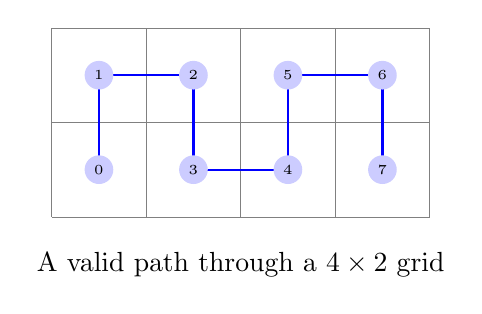
\begin{tikzpicture}[scale=1.2]
    \draw[step=1, gray, very thin] (0,0) grid (4,2);
    % A valid Hilbert-like path
    \draw[thick, blue, ->]
        (0.5,0.5) -- (0.5,1.5) -- (1.5,1.5) -- (1.5,0.5) --
        (2.5,0.5) -- (2.5,1.5) -- (3.5,1.5) -- (3.5,0.5);
    \foreach \x/\y/\n in {0.5/0.5/0, 0.5/1.5/1, 1.5/1.5/2, 1.5/0.5/3,
                          2.5/0.5/4, 2.5/1.5/5, 3.5/1.5/6, 3.5/0.5/7} {
        \node at (\x,\y) [circle, fill=blue!20, inner sep=2pt] {\tiny \n};
    }
    \node at (2, -0.5) {A valid path through a $4 \times 2$ grid};
\end{tikzpicture}
\end{center}
\begin{center}
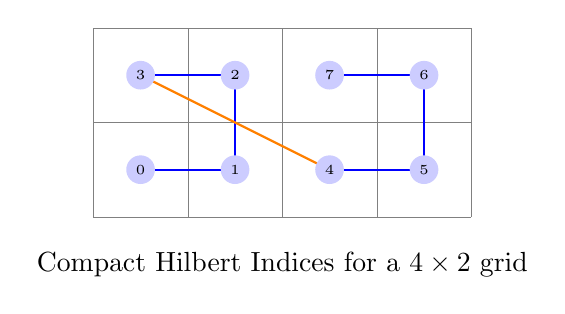
\begin{tikzpicture}[scale=1.2]
    \draw[step=1, gray, very thin] (0,0) grid (4,2);
    % A valid Hilbert-like path
    \draw[thick, blue, ->]
        (0.5,0.5) -- (1.5,0.5) -- (1.5,1.5) -- (0.5,1.5);
    \draw[thick, blue, ->]
        (2.5,0.5) -- (3.5,0.5) -- (3.5,1.5) -- (2.5,1.5);
    \draw[thick, orange, ->]
        (0.5,1.5) -- (2.5,0.5);
    \foreach \x/\y/\n in {0.5/0.5/0, 1.5/0.5/1, 1.5/1.5/2, 0.5/1.5/3,
                          2.5/0.5/4, 3.5/0.5/5, 3.5/1.5/6, 2.5/1.5/7} {
        \node at (\x,\y) [circle, fill=blue!20, inner sep=2pt] {\tiny \n};
    }
    \node at (2, -0.5) {Compact Hilbert Indices for a $4 \times 2$ grid};
\end{tikzpicture}
\end{center}

We see discontinuity in the compact Hilbert indices. This continuity can be helpful for
\begin{itemize}
    \item Using Hilbert curves to define bounding boxes.
    \item Using Hilbert curves for locality... I'll need to measure this.
    \item Using space-filling curves for CNC milling and laser cutting or for 3D printing.
    \item Data compression with change codes that encode only the next step direction.
    \item Image processing with the Riemersma dithering technique. You get jumps.
    \item Topological algorithms that detect connected components, as in "find all connected cloud pixels". Standard Hilbert also fragments regions, but lack of lattice continuity complicates stitching.
\end{itemize}
(There are Scan-line and Gilgamesh variants that are used for arbitrary rectangles for CNC.)

This article builds on the work of Hamilton and Rau-Chaplin to make a lattice-continuous Hilbert curve.


\section{Approaches to Space-Filling Curves}

Hamilton and Rao-Chaplin had a geometric approach to Hilbert curves.

There are more modern approaches to other space-filling curves.

Alternatives
\begin{itemize}
    \item Adaptive or scan-line by Zhang et al
    \item Psuedo-Hilbert curve
    \item Padding
\end{itemize}

\section{Preliminaries}

Let $m=[m_0,\ldots, m_{n-1}]$ define an $n$-dimensional discrete hyperrectangle $P(m)$ of extent
$[2^{m_0},\ldots,2^{m_{n-1}}]$. Let $M=\sum_j m_j$. The goal is to construct a bijection
$H_m\in [0, 2^M-1]\rightarrow P(m)$ such that $|H_m(h+1) - H_m(h)|_1=1$ for all $0\le h<2^M-1$.
The order of the Hilbert curve is $\order=\text{max}(m)$.

A level $\ell_s\in [1,\order]$ partitions the space of a discrete hypercube of size $[0,2^{\ell_s}]^n$ into $2^n$ sub-hypercubes. Those sub-hypercubes will have an index $i$ which Hamilton chose to be the well-known binary
reflected gray code $g(i)=i\XOR(\lfloor i/2 \rfloor)$.

The entry point $e(i)\in \{0, 1\}^n$ is the vertex of the $j$-th sub-hypercube where the curve
enters relative to the sub-hypercube's local coordinates.
\[
\entry(i) = \begin{cases}
0 & \text{if } i = 0 \\
\gc\left(2 \left\lfloor \frac{i-1}{2} \right\rfloor\right) & \text{if } i > 0
\end{cases}
\]
The direction to the exit point is
\[
\dir(i) = \begin{cases}
0 & \text{if } i = 0 \\
\mathrm{g}(i-1) \mod n & \text{if } i > 0 \text{ and } i \text{ is even} \\
\mathrm{g}(i) \mod n & \text{if } i \text{ is odd}
\end{cases}
\]
The exit point $\exitpt(i)$ relates to the entry point by
\[
    \exitpt(i)=\entry(i)\XOR 2^{\dir(i)}
\]

\section{Modified Derivation of Hilbert Indices}

Hamilton et al identified that the generic framework for Hilbert algorithms is to
\begin{enumerate}
    \item Find the cell containing the point of interest,
    \item Update the index value appropriately,
    \item Transform, and
    \item Recurse to the level below if needed.
\end{enumerate}
The idea of Hamilton and Rau-Chaplin was to identify \emph{active dimensions\/} at
each level so that updates and transforms applied only to the subset of active
dimensions. As the levels decrease and the grid is finer, there are more active
dimensions. They called this the \textsc{ExtractMask} step.

The step to recurse to the level below requires calculation of the entry point,
$e$ of the level below and the direction, $d$, from the entry to the exit, $f$, at the
level below.
\begin{align}
    e_{s-1} & = e_s\XOR(e_s(w)\ROTL d) \\
    d_{s-1} & = d_s + d(w) + 1\text{mod} n
\end{align}
These updates calulate the corner and direction one level down from the current level.

There is a problem with that update. The set of active axes one level down may be
greater than the set of active axes at the current level.


This is why that makes the result lattice-continuous.

Define the priority order $\prec$ on axes by $j \prec j'$ iff $(m_j, j) <{\text{lex}} (m{j'}, j')$.
  For each level $s$, let $A_s$ be the list of axes $j : m_j \ge s$ sorted in increasing $\prec$-order, with $k_s = |A_s|$.

\begin{definition}[Activation Embedding]
Given active axis lists $A = (a_0, \ldots, a_{k-1})$ and $A' = (a'_0, \ldots, a'_{k'-1})$
with $A \subseteq A'$, define $\mathrm{Embed}_{A \to A'}(e, d) = (e', d')$ where:
\begin{align}
e' &= \sum_{t=0}^{k-1} \bitfn(e, t) \cdot 2^{\mathrm{pos}_{A'}(a_t)} \\[4pt]
d' &= \mathrm{pos}_{A'}(a_d)
\end{align}
and $\mathrm{pos}_{A'}(j)$ denotes the position of axis $j$ in list $A'$.
\end{definition}


\subsection{The Encoding Algorithm}

\begin{algorithm}[H]
\caption{Encode: Point $\to$ Hilbert Index}
\begin{algorithmic}[1]
\Require Point $\mathbf{p} \in P(\mathbf{m})$
\Ensure Hilbert index $h \in \{0, \ldots, 2^M - 1\}$
\State $h \gets 0$
\State $e \gets 0$, $d \gets 0$ \Comment{Initial state: standard orientation}
\State Compute $A_s$ for all $s$ \Comment{Active axes sorted by $(m_j, j)$}
\For{$s = m_{\max}$ down to $1$}
    \State $k \gets k_s$ \Comment{Number of active axes at level $s$}
    \State $\ell \gets \sum_{t=0}^{k-1} \bitfn(p_{A[t]}, s-1) \cdot 2^t$ \Comment{Pack bits from active axes}
    \State $\bar{\ell} \gets T_{(e,d)}(k, \ell)$ \Comment{Apply orientation transform}
    \State $w \gets \gcinv(\bar{\ell})$ \Comment{Convert to sub-hypercube index}
    \State Append $w$ to $h$ \Comment{$h \gets h \cdot 2^k + w$}
    \State $e \gets e \XOR (\entry_k(w) \ROTL (d+1))$
    \State $d \gets (d + \dir_k(w) + 1) \mod k$

    \If{$k_{s-1} > k$} \Comment{Activation event: new axes become active}
        \State $(e', d') \gets \mathrm{Embed}_{A_s \to A_{s-1}}(e, d)$
    \EndIf
\EndFor
\State \Return $h$
\end{algorithmic}
\end{algorithm}

\section{Results}

Here is the change to the spatial locality.
Here is the change to the bounding box problem.

This paper has source code and an AI-generated proof-assistant derivation.



\end{document}
